\documentclass{article}

\usepackage{graphicx}
\usepackage{tikz}
\usepackage{tikzsymbols}
\usetikzlibrary{calc,patterns,shapes.geometric}
\pagestyle{empty}
\usepackage[margin=0pt]{geometry}
\geometry{papersize={14in,12in}}

\def\centerarc[#1](#2)(#3:#4:#5){\draw[#1] ($(#2)+({#5*cos(#3)},{#5*sin(#3)})$) arc (#3:#4:#5);}

\begin{document}
	\begin{figure}
		\centering
		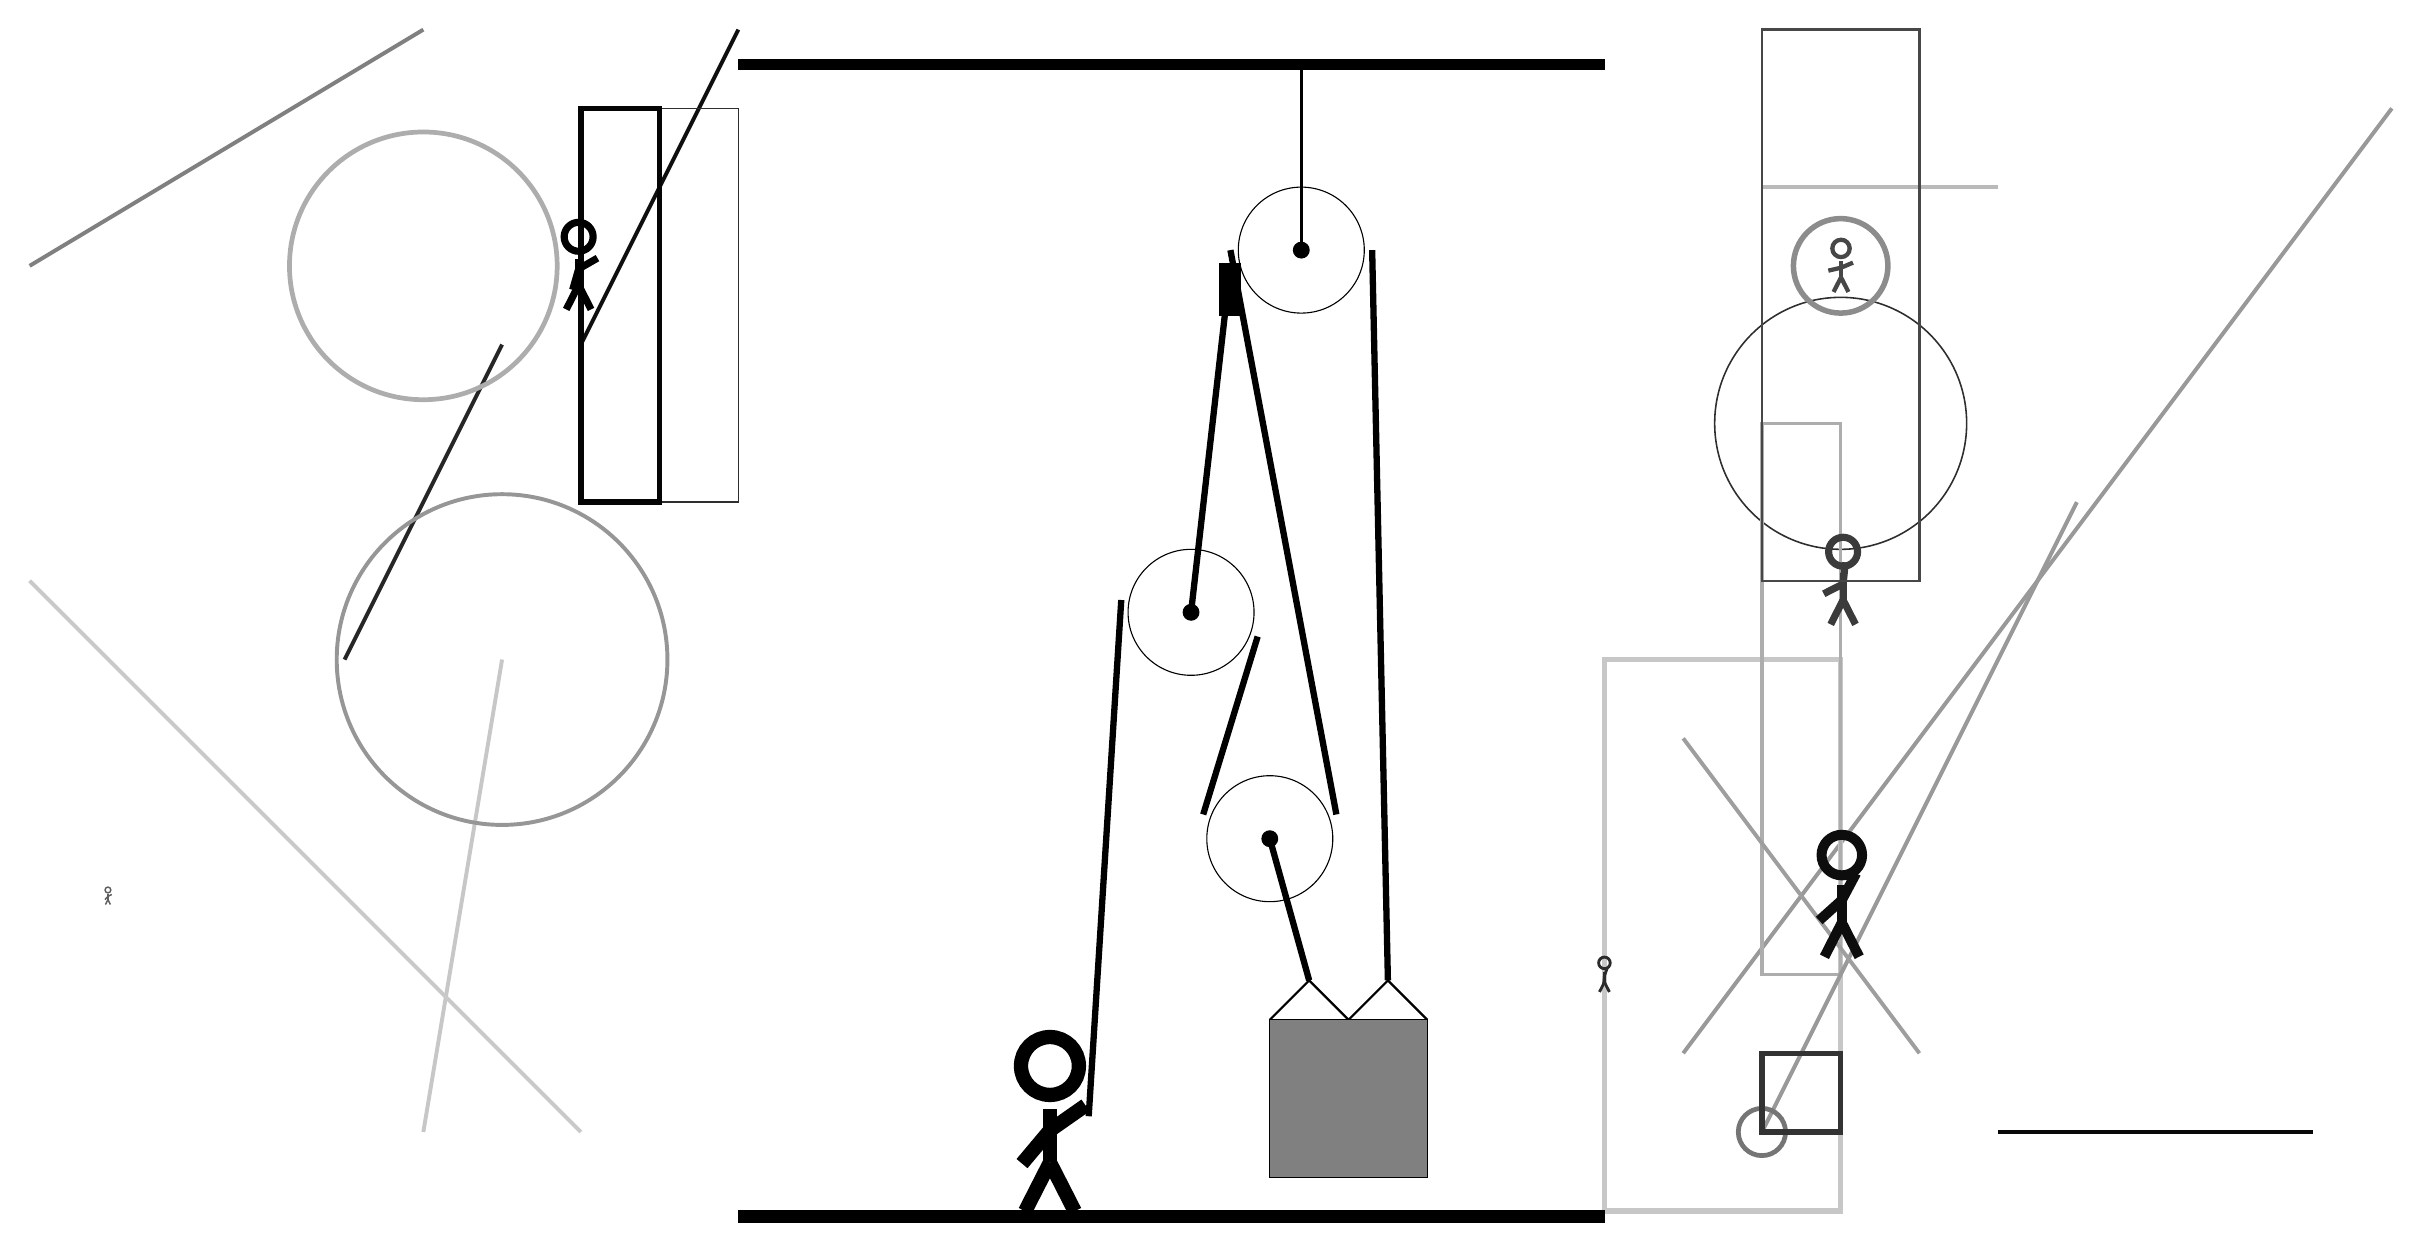
\begin{tikzpicture}
			%%%%% START %%%%%
			
			\draw[fill=black] (-6, 11.5) rectangle (5, 11.625);
			
			\draw[line width=0.5mm, color=black!97](10, -2) -- (14, -2);
			
			\draw[line width=0.5mm, color=black!40](6, -1) -- (15, 11);
			\draw [line width=0.2mm, color=black!82](8, 7) circle (1.6);
			\draw[line width=0.7mm, color=black!22] (5, 4) rectangle (8, -3);
			
			\draw[line width=0.5mm, color=black!94](-8, 8) -- (-6, 12);
			
			\draw[line width=0.2mm, color=black!82] (-6, 6) rectangle (-7, 11);
			
			\draw[line width=0.5mm, color=black!27](7, 10) -- (10, 10);
			\draw[line width=0.5mm, color=black!22](-10, -2) -- (-9, 4);
			\node[line width=0.4mm, color=black!83] at (5, 0) {\Strichmaxerl[2][85][70]};
			\draw[line width=0.4mm, color=black!32] (7, 7) rectangle (8, 0);
			
			\draw[line width=0.5mm, color=black!40](7, -2) -- (11, 6);
			\draw [line width=0.6mm, color=black!54](7, -2) circle (0.3);
			\draw[line width=0.5mm, color=black!50](-10, 12) -- (-15, 9);
			
			\draw[line width=0.5mm, color=black!38](9, -1) -- (6, 3);
			\draw[line width=0.5mm, color=black!21](-8, -2) -- (-15, 5);
			\node[line width=0.3mm, color=black!77] at (8, 5) {\Strichmaxerl[5][27][84]};
			
			\node[line width=0.4mm, color=black!72] at (8, 9) {\Strichmaxerl[3][13][23]};
			\draw[line width=0.5mm, color=black!85](-11, 4) -- (-9, 8);
			\draw[line width=0.7mm, color=black!80] (7, -2) rectangle (8, -1);
			
			\draw [line width=0.5mm, color=black!41](-9, 4) circle (2.1);
			\node[line width=0.2mm, color=black!63] at (-14, 1) {\Strichmaxerl[1][47][27]};
			
			\draw[line width=0.7mm, color=black!98] (-7, 6) rectangle (-8, 11);
			\node[line width=0.4mm, color=black!100] at (-8, 9) {\Strichmaxerl[5][74][30]};
			\draw [line width=0.7mm, color=black!45](8, 9) circle (0.6);
			\draw [line width=0.6mm, color=black!32](-10, 9) circle (1.7);
			
			\node[line width=0.7mm, color=black!95] at (8, 1) {\Strichmaxerl[7][42][62]};
			
			\draw[line width=0.3mm, color=black!72] (7, 12) rectangle (9, 5);
			
			\draw (-0.25, 4.6) circle (0.8);
			\draw[fill=black] (-0.25, 4.6) circle (0.1);
			
			\draw (0.75, 1.725) circle (0.8);
			\draw[fill=black] (0.75, 1.725) circle (0.1);
			
			\draw (1.15, 9.2) circle (0.8);
			\draw[fill=black] (1.15, 9.2) circle (0.1);
			\draw[very thick] (1.15, 9.2) -- (1.15, 11.5);
			
			\draw[thick]  (0.75, -0.575) -- (1.25, -0.075) -- (1.75, -0.575) -- (2.25, -0.075) -- (2.75, -0.575);
			\draw[fill=black!50] (0.75, -0.575) rectangle (2.75, -2.575);
			
			\draw[line width=0.8mm] (-0.25, 4.6) -- (0.25, 9.0);
			\draw[line width=0.8mm, fill=black](0.15, 8.4) rectangle (0.35, 9.0);
			\draw[line width=0.8mm] (-1.55, -1.8) -- (-1.1363, 4.7562);
			\centerarc[line width=0.8mm](-0.25, 4.6)(-20:170:0.9);
			\draw[line width=0.8mm] (0.5957, 4.2922) -- (-0.0957, 2.0328);
			\centerarc[line width=0.8mm](0.75, 1.725)(160:380:0.9);
			\draw[line width=0.8mm] (1.5957, 2.0328) -- (0.25, 9.2);
			\draw[line width=0.8mm](0.75, 1.725) -- (1.25, -0.075);
			\centerarc[line width=0.8mm](1.15, 9.2)(0:180:0.9);
			\draw[line width=0.8mm] (2.05, 9.2) -- (2.25, -0.075);
			
			\node at (-2, -1.9) {\Strichmaxerl[10][50][35]};
			
			\draw[fill=black] (-6, -3) rectangle (5, -3.15);
			
			%%%%% END %%%%%
		\end{tikzpicture}
	\end{figure}	
\end{document}